% Fig.1: Kunai architecture — inputs, compiler pipeline, and the
% host BPF program that embeds the generated bytecode.
% Vertical flow, sized for a one-column figure.
% Build: pdflatex fig_arch.tex -> fig_arch.pdf
\documentclass[tikz]{standalone}
\usetikzlibrary{positioning, arrows.meta, fit, calc}
\begin{document}
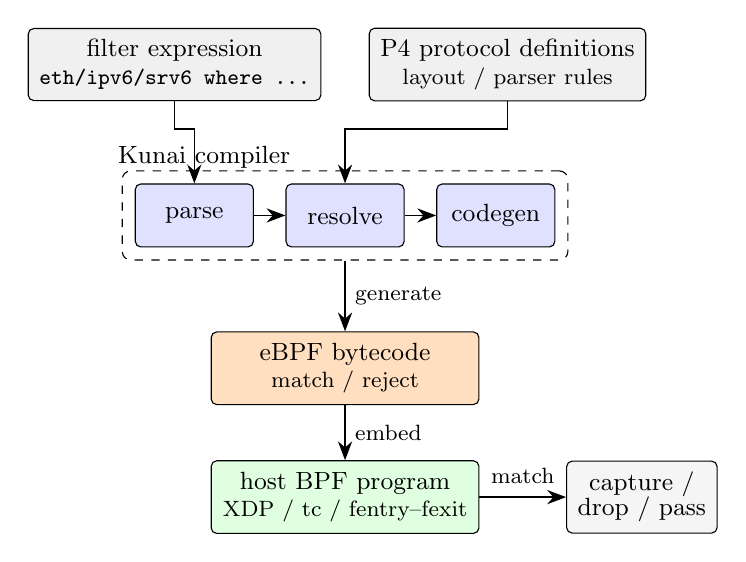
\begin{tikzpicture}[
  font=\small,
  box/.style={draw, rounded corners=2pt, align=center, inner sep=4pt, minimum height=8mm},
  input/.style={box, fill=gray!12},
  stage/.style={box, fill=blue!12, minimum width=15mm},
  bcbox/.style={box, fill=orange!25, minimum width=34mm},
  host/.style={box, fill=green!12, minimum width=34mm},
  arr/.style={-{Stealth[length=2.4mm]}, semithick},
]

% --- inputs (top row) ---
\node[input, minimum width=30mm] (expr) at (0,0)
  {filter expression\\[-1pt] {\footnotesize\texttt{eth/ipv6/srv6 where ...}}};
\node[input, minimum width=30mm, right=6mm of expr] (vocab)
  {P4 protocol definitions\\[-1pt] {\footnotesize layout / parser rules}};

% --- compiler pipeline ---
\node[stage] (resolve) at ($(expr.south east)!0.5!(vocab.south west) + (0,-1.45)$) {resolve};
\node[stage, left=4mm of resolve] (parse) {parse};
\node[stage, right=4mm of resolve] (codegen) {codegen};
\node[draw, dashed, rounded corners=3pt, inner sep=4.5pt,
      fit=(parse)(resolve)(codegen),
      label={[font=\small, yshift=-1mm]above left:Kunai compiler}] (compiler) {};

% --- output bytecode ---
\node[bcbox, below=9mm of compiler] (bc)
  {eBPF bytecode\\[-1pt] {\footnotesize match / reject}};

% --- host program ---
\node[host, below=7mm of bc] (hostprog)
  {host BPF program\\[-1pt] {\footnotesize XDP / tc / fentry--fexit}};
\node[box, fill=gray!8, right=11mm of hostprog, align=center] (act)
  {capture /\\[-2pt] drop / pass};

% --- arrows ---
\draw[arr] (expr.south) -- ++(0,-3.5mm) -| (parse.north);
\draw[arr] (vocab.south) -- ++(0,-3.5mm) -| (resolve.north);
\draw[arr] (parse) -- (resolve);
\draw[arr] (resolve) -- (codegen);
\draw[arr] (compiler.south) -- node[right, font=\footnotesize] {generate} (bc.north);
\draw[arr] (bc.south) -- node[right, font=\footnotesize] {embed} (hostprog.north);
\draw[arr] (hostprog.east) -- node[above=0.5mm, font=\footnotesize] {match} (act.west);

\end{tikzpicture}
\end{document}
